\documentclass[11pt,a4paper]{report}
\usepackage[textwidth=37em,vmargin=30mm]{geometry}
\usepackage{calc,xunicode,amsmath,amssymb,paralist,enumitem,tabu,booktabs,datetime2,xeCJK,xeCJKfntef,listings}
\usepackage{tocloft,fancyhdr,tcolorbox,xcolor,graphicx,eso-pic,xltxtra,xelatexemoji}

\newcommand{\envyear}[0]{2025}
\newcommand{\envdatestr}[0]{2025-01-23}
\newcommand{\envfinaldir}[0]{webdb/2025/20250123/final}

\usepackage[hidelinks]{hyperref}
\hypersetup{
    colorlinks=false,
    pdfpagemode=FullScreen,
    pdftitle={Web Digest - \envdatestr}
}

\setlength{\cftbeforechapskip}{10pt}
\renewcommand{\cftchapfont}{\rmfamily\bfseries\large\raggedright}
\setlength{\cftbeforesecskip}{2pt}
\renewcommand{\cftsecfont}{\sffamily\small\raggedright}

\setdefaultleftmargin{2em}{2em}{1em}{1em}{1em}{1em}

\usepackage{xeCJK,xeCJKfntef}
\xeCJKsetup{PunctStyle=plain,RubberPunctSkip=false,CJKglue=\strut\hskip 0pt plus 0.1em minus 0.05em,CJKecglue=\strut\hskip 0.22em plus 0.2em}
\XeTeXlinebreaklocale "zh"
\XeTeXlinebreakskip = 0pt


\setmainfont{Brygada 1918}
\setromanfont{Brygada 1918}
\setsansfont{IBM Plex Sans}
\setmonofont{JetBrains Mono NL}
\setCJKmainfont{Noto Serif CJK SC}
\setCJKromanfont{Noto Serif CJK SC}
\setCJKsansfont{Noto Sans CJK SC}
\setCJKmonofont{Noto Sans CJK SC}

\setlength{\parindent}{0pt}
\setlength{\parskip}{8pt}
\linespread{1.15}

\lstset{
	basicstyle=\ttfamily\footnotesize,
	numbersep=5pt,
	backgroundcolor=\color{black!5},
	showspaces=false,
	showstringspaces=false,
	showtabs=false,
	tabsize=2,
	captionpos=b,
	breaklines=true,
	breakatwhitespace=true,
	breakautoindent=true,
	linewidth=\textwidth
}






\newcommand{\coverpic}[2]{
    % argv: itemurl, authorname
    Cover photo by #2~~(\href{#1}{#1})
}
\newcommand{\makeheader}[0]{
    \begin{titlepage}
        % \newgeometry{hmargin=15mm,tmargin=21mm,bmargin=12mm}
        \begin{center}
            
            \rmfamily\scshape
            \fontspec{BaskervilleF}
            \fontspec{Old Standard}
            \fontsize{59pt}{70pt}\selectfont
            WEB\hfill DIGEST
            
            \vfill
            % \vskip 30pt
            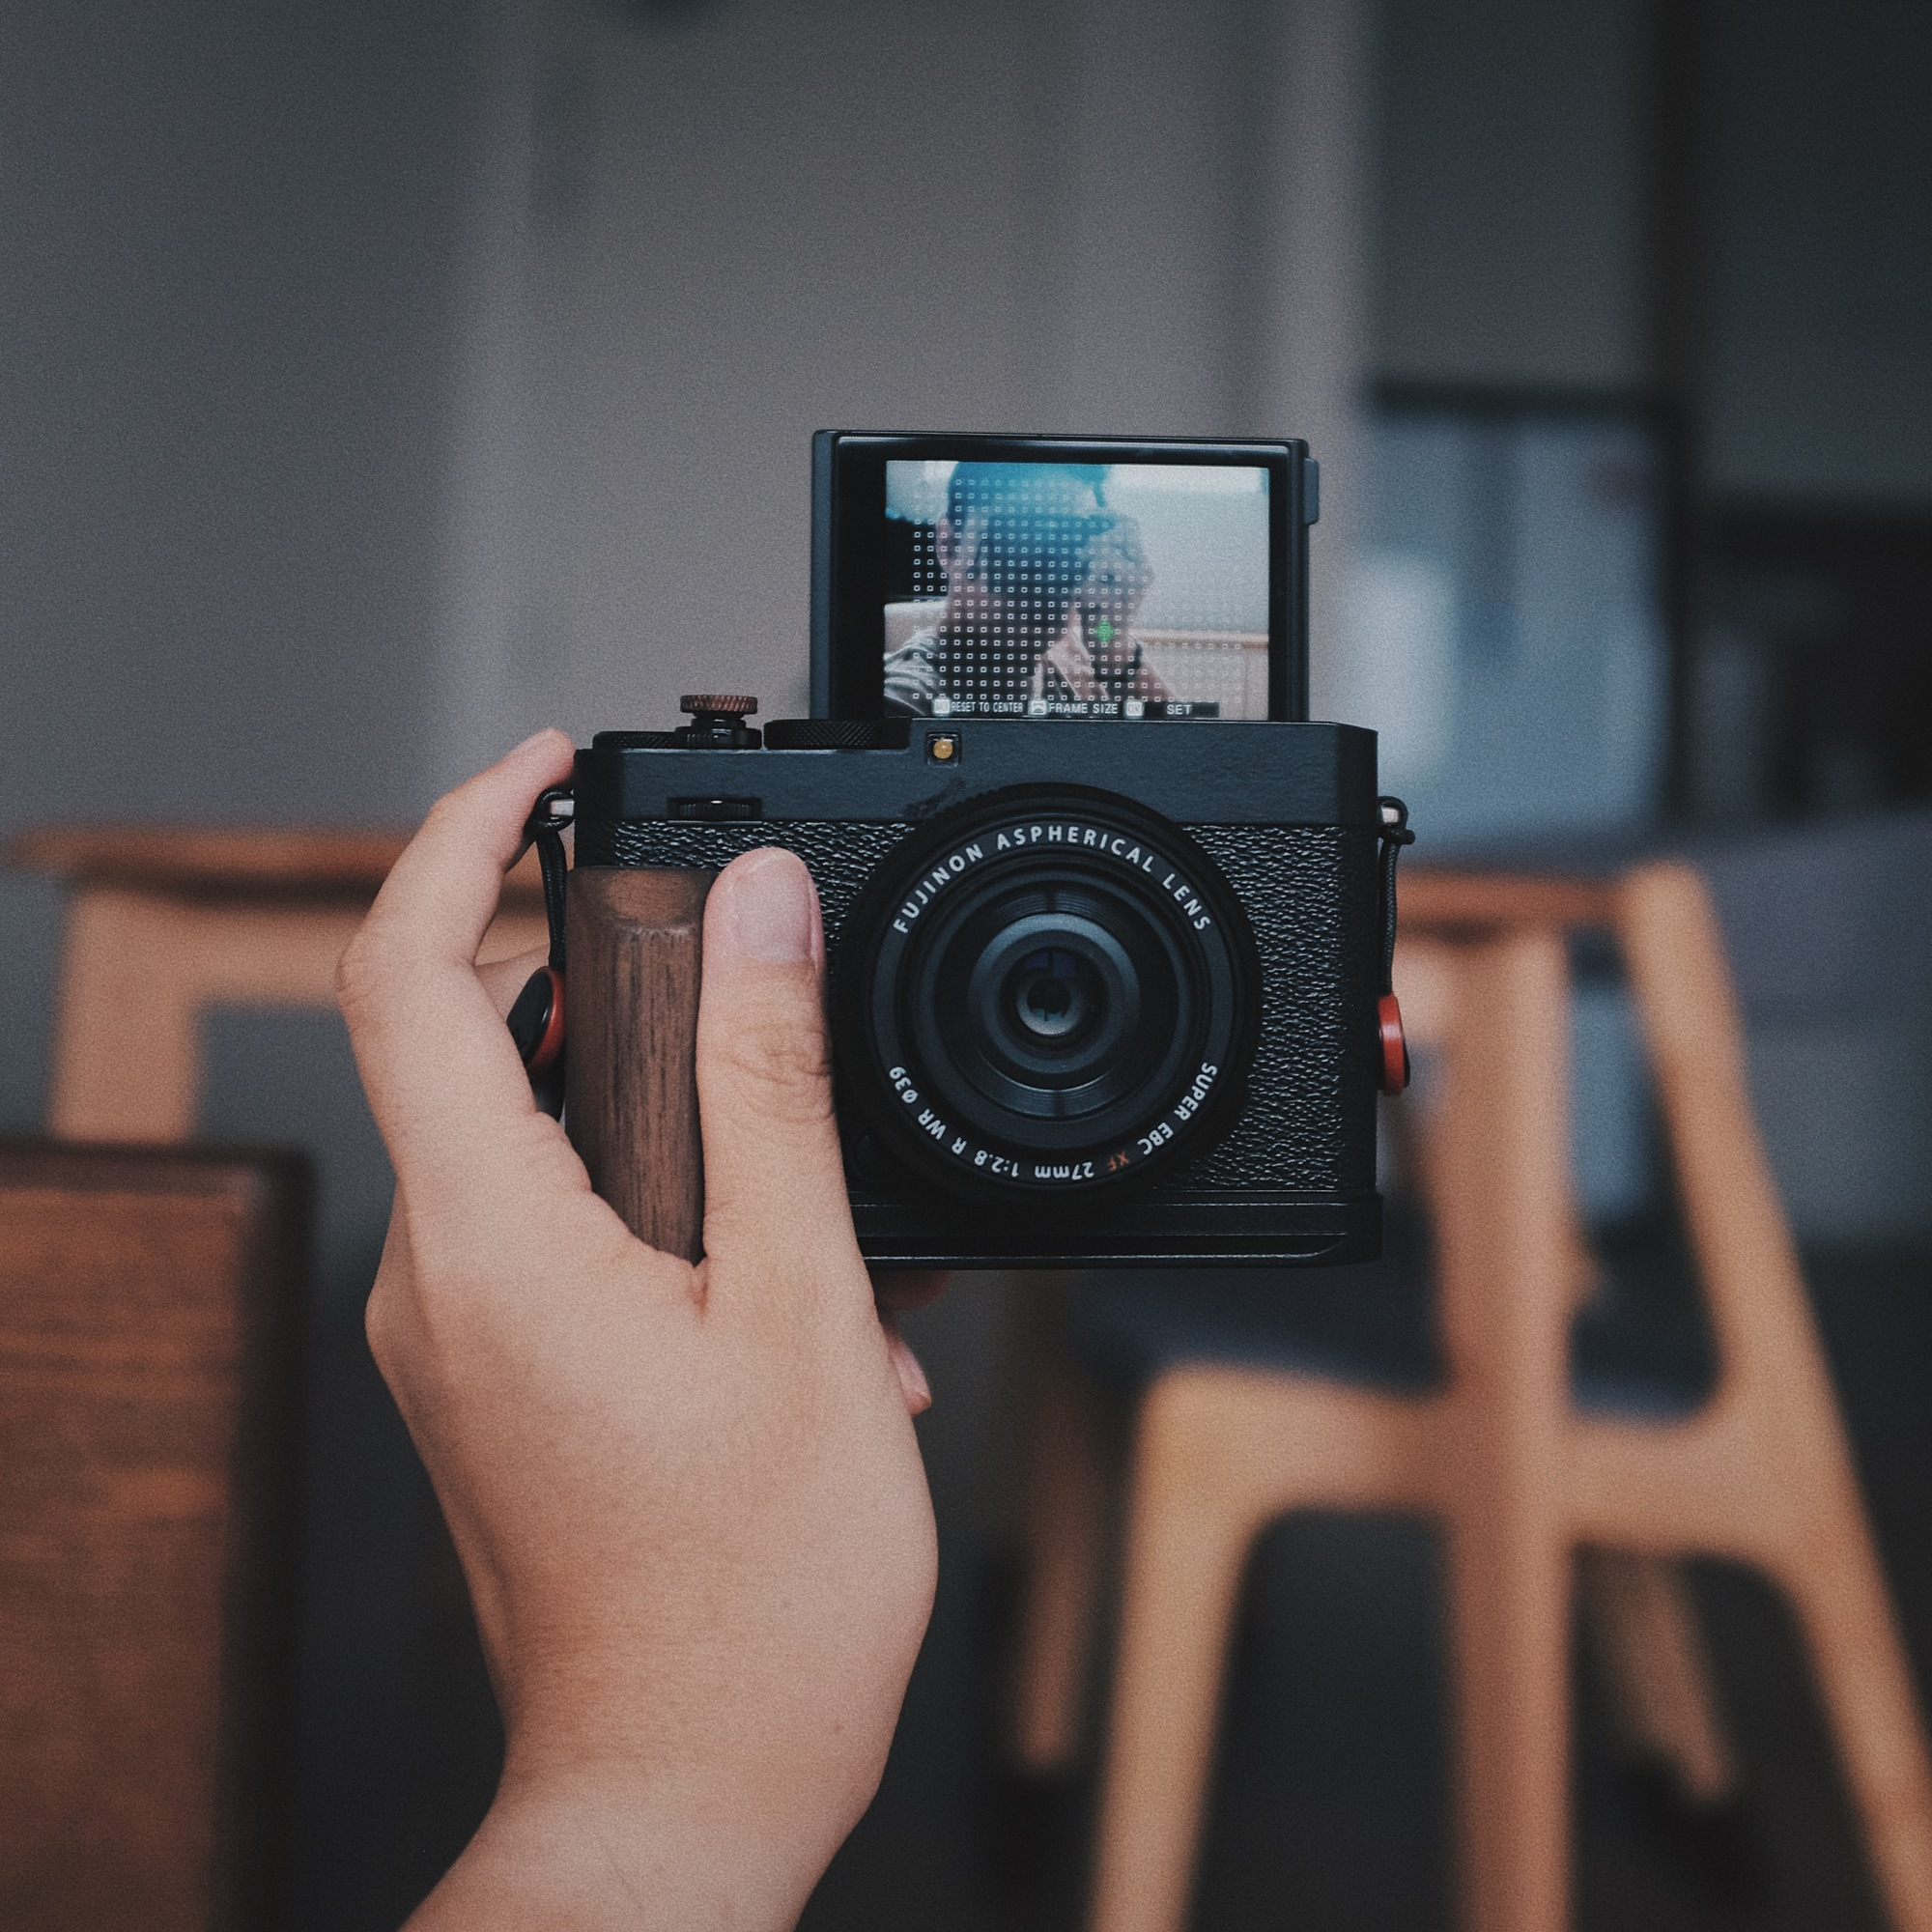
\includegraphics[width=\linewidth]{\envfinaldir/coverpic-prod.jpg}\par
            % \vskip 30pt
            \vfill

            \normalsize\rmfamily\scshape
            \copyright{} The Web Digest Project \hfill\large \envdatestr
        \end{center}
    \end{titlepage}
    % \restoregeometry
}
\newcommand{\simplehref}[1]{%
    \textcolor{blue!80!green}{\href{#1}{#1}}%
}
\renewcommand{\contentsname}{\center\Huge\sffamily\bfseries Contents\par\vskip 20pt}
\newcounter{ipartcounter}
\setcounter{ipartcounter}{0}
\newcommand{\ipart}[1]{
    % \vskip 20pt
    \clearpage
    \stepcounter{ipartcounter}
    \phantomsection
    \addcontentsline{toc}{chapter}{#1}
    % \begin{center}
    %     \Huge
    %     \sffamily\bfseries
    %     #1
    % \end{center}
    % \vskip 20pt plus 7pt
}
\newcounter{ichaptercounter}
\setcounter{ichaptercounter}{0}
\newcommand{\ichapter}[1]{
    % \vskip 20pt
    \clearpage
    \stepcounter{ichaptercounter}
    \phantomsection
    \addcontentsline{toc}{section}{\numberline{\arabic{ichaptercounter}}#1}
    \begin{center}
        \Huge
        \sffamily\bfseries
        #1
    \end{center}
    \vskip 20pt plus 7pt
}
\newcommand{\entrytitlefont}[1]{\subsection*{\raggedright\Large\sffamily\bfseries#1}}
\newcommand{\entryitemGeneric}[2]{
    % argv: title, url
    \parbox{\linewidth}{
        \entrytitlefont{#1}\par\vskip 5pt
        \footnotesize\ttfamily\mdseries
        \simplehref{#2}
    }\vskip 11pt plus 11pt minus 1pt
}
\newcommand{\entryitemGithub}[3]{
    % argv: title, url, desc
    \parbox{\linewidth}{
        \entrytitlefont{#1}\par\vskip 5pt
        \footnotesize\ttfamily\mdseries
        \simplehref{#2}\par\vskip 5pt
        \small\rmfamily\mdseries#3
    }\vskip 11pt plus 11pt minus 1pt
}
\newcommand{\entryitemAp}[3]{
    % argv: title, url, desc
    \parbox{\linewidth}{
        \entrytitlefont{#1}\par\vskip 5pt
        \footnotesize\ttfamily\mdseries
        \simplehref{#2}\par\vskip 5pt
        \small\rmfamily\mdseries#3
    }\vskip 11pt plus 11pt minus 1pt
}
\newcommand{\entryitemHackernews}[3]{
    % argv: title, hnurl, rawurl
    % \parbox{\linewidth}{
    %     \entrytitlefont{#1}\par\vskip 5pt
    %     \footnotesize\ttfamily\mdseries
    %     \simplehref{#3}\par
    %     \textcolor{black!50}{\href{#2}{#2}}
    % }\vskip 11pt plus 11pt minus 1pt
    \begin{minipage}{\linewidth}
            \entrytitlefont{#1}\par\vskip 5pt
            \footnotesize\ttfamily\mdseries
            \simplehref{#3}\par
            \textcolor{black!50}{\href{#2}{#2}}
    \end{minipage}\par\vskip 11pt plus 11pt minus 1pt
}







\begin{document}

\makeheader

\tableofcontents\clearpage




\ipart{Developers}
\ichapter{Hacker News}
\entryitemTwoLinks{Show HN: I Made an Open-Source Laptop from Scratch}{https://news.ycombinator.com/item?id=42797260}{https://www.byran.ee/posts/creation/}

\entryitemTwoLinks{How to improve your WFH lighting to reduce eye strain}{https://news.ycombinator.com/item?id=42796950}{https://rustle.ca/posts/articles/work-from-home-lighting}

\entryitemTwoLinks{C stdlib isn't threadsafe and even safe Rust didn't save us}{https://news.ycombinator.com/item?id=42796058}{https://www.edgedb.com/blog/c-stdlib-isn-t-threadsafe-and-even-safe-rust-didn-t-save-us}

\entryitemTwoLinks{TabBoo – add random jumpscares to websites you're trying to avoid}{https://news.ycombinator.com/item?id=42795237}{https://tabboo.xyz/}

\entryitemTwoLinks{Minimal 64x4 Home Computer}{https://news.ycombinator.com/item?id=42794232}{https://github.com/slu4coder/Minimal-64x4-Home-Computer}

\entryitemTwoLinks{Mastercard DNS error went unnoticed for years}{https://news.ycombinator.com/item?id=42793783}{https://krebsonsecurity.com/2025/01/mastercard-dns-error-went-unnoticed-for-years/}

\entryitemTwoLinks{Show HN: Stratoshark, a sibling application to Wireshark}{https://news.ycombinator.com/item?id=42793777}{https://stratoshark.org/}

\entryitemTwoLinks{Simple CPU Design}{https://news.ycombinator.com/item?id=42793597}{http://simplecpudesign.com/}

\entryitemTwoLinks{OpenAI has upped its lobbying efforts nearly sevenfold}{https://news.ycombinator.com/item?id=42793567}{https://www.technologyreview.com/2025/01/21/1110260/openai-ups-its-lobbying-efforts-nearly-seven-fold/}

\entryitemTwoLinks{The Tyranny of Structurelessness (1970)}{https://news.ycombinator.com/item?id=42793483}{https://www.jofreeman.com/joreen/tyranny.htm}

\entryitemTwoLinks{Show HN: NotepadJs – A cross-platform love letter to Notepad}{https://news.ycombinator.com/item?id=42791820}{https://github.com/itamarom/notepadjs}

\entryitemTwoLinks{My Struggle with Doom Scrolling}{https://news.ycombinator.com/item?id=42791428}{https://allthatjazz.me/posts/doom-scrolling-struggles}

\entryitemTwoLinks{The Day Instagram Blocked Democracy}{https://news.ycombinator.com/item?id=42790729}{https://docpop.org/2025/01/the-day-instagram-blocked-democracy/}

\entryitemTwoLinks{DHS removes all members of cyber security advisory boards, halts investigations}{https://news.ycombinator.com/item?id=42790207}{https://bsky.app/profile/ericjgeller.com/post/3lgbpqmxeok2f}

\entryitemTwoLinks{Flame: A small language model for spreadsheet formulas (2023)}{https://news.ycombinator.com/item?id=42788580}{https://arxiv.org/abs/2301.13779}

\entryitemTwoLinks{What are these bumps on the top of a pull-tab can?}{https://news.ycombinator.com/item?id=42788455}{https://old.reddit.com/r/whatisthisthing/comments/1i5ztq4/comment/m8a7m8m/}

\entryitemTwoLinks{Tensor Product Attention Is All You Need}{https://news.ycombinator.com/item?id=42788451}{https://arxiv.org/abs/2501.06425}

\entryitemTwoLinks{Why is zero plural? (2024)}{https://news.ycombinator.com/item?id=42787651}{https://ell.stackexchange.com/questions/352455/why-is-zero-plural}

\entryitemTwoLinks{Isolating complexity is the essence of successful abstractions}{https://news.ycombinator.com/item?id=42787531}{https://v5.chriskrycho.com/journal/essence-of-successful-abstractions/}

\entryitemTwoLinks{Ross Ulbricht granted a full pardon}{https://news.ycombinator.com/item?id=42786962}{https://twitter.com/Free\_Ross/status/1881851923005165704}\ichapter{Phoronix}
\entryitemGeneric{\hskip 0pt{}Intel Calls For More Modular PC Designs, Easier Component Replacement/Upgrades}{https://www.phoronix.com/news/Intel-More-Modular-PC-Designs}

\entryitemGeneric{\hskip 0pt{}Arch Linux Installer Adds Wayfire As A Desktop Option, Btrfs Improvements}{https://www.phoronix.com/news/Arch-Linux-Archinstall-3.0.2}

\entryitemGeneric{\hskip 0pt{}Free Software Foundation Marking 40 Years Old With A New Logo}{https://www.phoronix.com/news/Free-Software-FSF-40-Year-Logo}

\entryitemGeneric{\hskip 0pt{}AMD Radeon On Linux 6.13 + Mesa 25.0-devel vs. NVIDIA R565 Linux Graphics/Gaming Performance}{https://www.phoronix.com/review/jan2025-linux-gpus}

\entryitemGeneric{\hskip 0pt{}AMD Announces The AMDGPU Composition Stack "ACS" For Advanced Linux Desktop Features}{https://www.phoronix.com/news/AMD-AMDGPU-Composition-Stack}

\entryitemGeneric{\hskip 0pt{}Very Promising Linux Patch Optimizes TLB Flushes During Page Reclamation}{https://www.phoronix.com/news/Linux-Optimize-TLB-Flush-Reclaim}

\entryitemGeneric{\hskip 0pt{}Linux's KUnit Will Now Default To Using Hardware Acceleration For Faster Testing}{https://www.phoronix.com/news/Linux-KUnit-Hardware-Accel}

\entryitemGeneric{\hskip 0pt{}Linux 6.14 Working To Make It Less Painful Debugging Early Boot Issues}{https://www.phoronix.com/news/Linux-6.14-Early-Boot-Debugging}

\entryitemGeneric{\hskip 0pt{}AMD Releases Orochi 3.0 For HIP \& CUDA API Switching At Run-Time}{https://www.phoronix.com/news/AMD-Orochi-3.0}\ichapter{Dribbble}
\entryitemGeneric{\hskip 0pt{}Carbon Solutions B2B Dashboard Design}{https://dribbble.com/shots/25506638-Carbon-Solutions-B2B-Dashboard-Design}

\entryitemGeneric{\hskip 0pt{}Bestest Brand®}{https://dribbble.com/shots/25510300-Bestest-Brand}

\entryitemGeneric{\hskip 0pt{}QVELTY / Design \& Animation}{https://dribbble.com/shots/25507639-QVELTY-Design-Animation}

\entryitemGeneric{\hskip 0pt{}Haptic Logo Design}{https://dribbble.com/shots/25504012-Haptic-Logo-Design}

\entryitemGeneric{\hskip 0pt{}Wine Label}{https://dribbble.com/shots/25509757-Wine-Label}

\entryitemGeneric{\hskip 0pt{}Letter V + LED + Wires Logo}{https://dribbble.com/shots/25507506-Letter-V-LED-Wires-Logo}

\entryitemGeneric{\hskip 0pt{}Robin bird logo}{https://dribbble.com/shots/25509208-Robin-bird-logo}

\entryitemGeneric{\hskip 0pt{}Qore - Logo Design}{https://dribbble.com/shots/25509466-Qore-Logo-Design}

\entryitemGeneric{\hskip 0pt{}Wine Label}{https://dribbble.com/shots/25503830-Wine-Label}

\entryitemGeneric{\hskip 0pt{}Monocle Cat}{https://dribbble.com/shots/25502155-Monocle-Cat}

\entryitemGeneric{\hskip 0pt{}Roundrobin}{https://dribbble.com/shots/25502404-Roundrobin}

\entryitemGeneric{\hskip 0pt{}"Nature Morte" - Promotional piece}{https://dribbble.com/shots/25501105--Nature-Morte-Promotional-piece}

\entryitemGeneric{\hskip 0pt{}Fitness App Design}{https://dribbble.com/shots/25494068-Fitness-App-Design}

\entryitemGeneric{\hskip 0pt{}Personal Banking App}{https://dribbble.com/shots/25493958-Personal-Banking-App}

\entryitemGeneric{\hskip 0pt{}404}{https://dribbble.com/shots/25492419-404}

\entryitemGeneric{\hskip 0pt{}Wine Label}{https://dribbble.com/shots/25490604-Wine-Label}

\entryitemGeneric{\hskip 0pt{}planet}{https://dribbble.com/shots/25490310-planet}

\entryitemGeneric{\hskip 0pt{}Shihiko // E-commerce Website}{https://dribbble.com/shots/25489208-Shihiko-E-commerce-Website}

\entryitemGeneric{\hskip 0pt{}Lonely Capybara}{https://dribbble.com/shots/25489946-Lonely-Capybara}

\entryitemGeneric{\hskip 0pt{}Wine Label}{https://dribbble.com/shots/25485370-Wine-Label}

\entryitemGeneric{\hskip 0pt{}Roam Supply Co. - Shirt Graphic}{https://dribbble.com/shots/25433659-Roam-Supply-Co-Shirt-Graphic}

\entryitemGeneric{\hskip 0pt{}EA System Ambigram}{https://dribbble.com/shots/25486215-EA-System-Ambigram}

\entryitemGeneric{\hskip 0pt{}Aquascaping Logos 🐠}{https://dribbble.com/shots/25486067-Aquascaping-Logos}

\entryitemGeneric{\hskip 0pt{}Botanica web}{https://dribbble.com/shots/25481584-Botanica-web}


\ipart{Developers~~~~(zh-Hans)}
\ichapter{Solidot}
\entryitemGeneric{\hskip 0pt{}过去一个世纪男性身高体重增长速度两倍于女性}{https://www.solidot.org/story?sid=80399}

\entryitemGeneric{\hskip 0pt{}杭州深度求索发布能挑战 OpenAI o1 的推理模型 DeepSeek R1}{https://www.solidot.org/story?sid=80398}

\entryitemGeneric{\hskip 0pt{}黑猩猩的撒尿行为具有传染性}{https://www.solidot.org/story?sid=80397}

\entryitemGeneric{\hskip 0pt{}耐药菌在乌克兰扩散}{https://www.solidot.org/story?sid=80396}

\entryitemGeneric{\hskip 0pt{}中国 2024 年可更新能源装机容量再创记录}{https://www.solidot.org/story?sid=80395}

\entryitemGeneric{\hskip 0pt{}Wine 10.0 释出}{https://www.solidot.org/story?sid=80394}

\entryitemGeneric{\hskip 0pt{}TikTok 被指限制反特朗普关键词的搜索}{https://www.solidot.org/story?sid=80393}

\entryitemGeneric{\hskip 0pt{}IMDb 创始人卸任 CEO 一职}{https://www.solidot.org/story?sid=80392}

\entryitemGeneric{\hskip 0pt{}特朗普赦免 Ross Ulbricht}{https://www.solidot.org/story?sid=80391}

\entryitemGeneric{\hskip 0pt{}北京将举办首届人机马拉松}{https://www.solidot.org/story?sid=80390}

\entryitemGeneric{\hskip 0pt{}X、Facebook、Instagram 和 YouTube 向欧盟承诺处理仇恨言论}{https://www.solidot.org/story?sid=80389}

\entryitemGeneric{\hskip 0pt{}干旱愈来愈严重愈来愈频繁}{https://www.solidot.org/story?sid=80388}

\entryitemGeneric{\hskip 0pt{}愈来愈多的美国青少年使用 ChatGPT 完成作业 }{https://www.solidot.org/story?sid=80387}

\entryitemGeneric{\hskip 0pt{}Paul Allen 诞辰 72 周年}{https://www.solidot.org/story?sid=80386}

\entryitemGeneric{\hskip 0pt{}孕妇的脑灰质在孕期发生变化}{https://www.solidot.org/story?sid=80385}

\entryitemGeneric{\hskip 0pt{}佳能的直播应用不支持佳能摄像机}{https://www.solidot.org/story?sid=80384}

\entryitemGeneric{\hskip 0pt{}华为 2024 年手机出货量增长 50\%}{https://www.solidot.org/story?sid=80383}

\entryitemGeneric{\hskip 0pt{}2024 年大气二氧化碳增幅创纪录}{https://www.solidot.org/story?sid=80382}

\entryitemGeneric{\hskip 0pt{}欧盟考虑在消费品中禁止使用 PFAS}{https://www.solidot.org/story?sid=80381}

\entryitemGeneric{\hskip 0pt{}Google 搜索服务开始要求启用 JavaScript}{https://www.solidot.org/story?sid=80380}\ichapter{V2EX}
\entryitemGeneric{\hskip 0pt{}[阅读] 2024 年读书总结}{https://www.v2ex.com/t/1107215}

\entryitemGeneric{\hskip 0pt{}[Docker] 有哪些简单的国内可用的免费的 docker 私有镜像仓库?}{https://www.v2ex.com/t/1107214}

\entryitemGeneric{\hskip 0pt{}[分享发现] 教你在 5 分钟之内和心仪女生开始交往}{https://www.v2ex.com/t/1107213}

\entryitemGeneric{\hskip 0pt{}[程序员] 请教一下各位大佬关于小说平台后端方案问题。}{https://www.v2ex.com/t/1107212}

\entryitemGeneric{\hskip 0pt{}[Microsoft Office] 如何解决 macOS 下 Office365 丢失登录状态,每次打开都要求登录}{https://www.v2ex.com/t/1107211}

\entryitemGeneric{\hskip 0pt{}[OpenWrt] 在 openwrt 下,配置 80211r 实现 AP 节点漫游}{https://www.v2ex.com/t/1107210}

\entryitemGeneric{\hskip 0pt{}[程序员] 求推荐动态 HTTP 或 S5 代理 爬虫用}{https://www.v2ex.com/t/1107209}

\entryitemGeneric{\hskip 0pt{}[问与答] m2 mac mini 和 零刻 EQ13 如何分配?}{https://www.v2ex.com/t/1107208}

\entryitemGeneric{\hskip 0pt{}[分享发现] 美国宣布 5000 亿美元``星际门''人工智能基础设施项目:甲骨文创始人、软银创始人、OpenAI 创始人}{https://www.v2ex.com/t/1107207}

\entryitemGeneric{\hskip 0pt{}[Apple] Apple Pencil Pro 官网演示侧旋用的是哪款 APP?}{https://www.v2ex.com/t/1107206}

\entryitemGeneric{\hskip 0pt{}[生活] 现在话费起充都是 50 了?}{https://www.v2ex.com/t/1107205}

\entryitemGeneric{\hskip 0pt{}[宽带症候群] 因为房东不让拉宽带,买了一台最强的 CPE\_5G 路由!(测试结果)}{https://www.v2ex.com/t/1107204}

\entryitemGeneric{\hskip 0pt{}[Apple] 图形程序员是否需要 Macbook Pro M4?}{https://www.v2ex.com/t/1107202}

\entryitemGeneric{\hskip 0pt{}[Android] 求助帖: Android Framework 的前景?}{https://www.v2ex.com/t/1107201}

\entryitemGeneric{\hskip 0pt{}[Apple] iOS 模拟器调试工具 RocketSim 限时活动}{https://www.v2ex.com/t/1107200}

\entryitemGeneric{\hskip 0pt{}[酷工作] 招聘高级 Unity 开发工程师}{https://www.v2ex.com/t/1107198}

\entryitemGeneric{\hskip 0pt{}[分享创造] 🎨 SVG 在线转换工具}{https://www.v2ex.com/t/1107197}

\entryitemGeneric{\hskip 0pt{}[问与答] Trae 的 UI 配色方案挺好啊,有大神能移植到 Vscode 或者 Cursor 上吗?}{https://www.v2ex.com/t/1107196}

\entryitemGeneric{\hskip 0pt{}[程序员] 手贱拿大模型试了下最近一次的 LeetCode 周赛,道心破碎了,成仙路已断,前路在何方?}{https://www.v2ex.com/t/1107195}

\entryitemGeneric{\hskip 0pt{}[Windows] windows 更新后好像固定在任务栏的 chrome 消失了?}{https://www.v2ex.com/t/1107194}

\entryitemGeneric{\hskip 0pt{}[NAS] 如何使用 Docker 一键部署 qBittorrent}{https://www.v2ex.com/t/1107193}

\entryitemGeneric{\hskip 0pt{}[Java] update 大家会允许这样写吗?}{https://www.v2ex.com/t/1107192}

\entryitemGeneric{\hskip 0pt{}[宽带症候群] 0755 公网 ip 封 bt 端口}{https://www.v2ex.com/t/1107191}

\entryitemGeneric{\hskip 0pt{}[程序员] 吐槽一下 b 站的推荐}{https://www.v2ex.com/t/1107190}

\entryitemGeneric{\hskip 0pt{}[酷工作] [web3] [远程办公] AI 算法产品团队搭建,也有其他开发,业务岗}{https://www.v2ex.com/t/1107187}

\entryitemGeneric{\hskip 0pt{}[Linux] wine 10.0 发布了}{https://www.v2ex.com/t/1107186}

\entryitemGeneric{\hskip 0pt{}[问与答] 有没有通用的办法 根据一个 dy/xhs 视频逆向搜用户 id?}{https://www.v2ex.com/t/1107185}

\entryitemGeneric{\hskip 0pt{}[分享发现] 做网站就做网站,写前端就写前端,可以不说 cursor 了吗}{https://www.v2ex.com/t/1107184}

\entryitemGeneric{\hskip 0pt{}[程序员] 简单聊聊我的 10 年程序员经历,微博,滴滴,爱彼迎}{https://www.v2ex.com/t/1107183}

\entryitemGeneric{\hskip 0pt{}[程序员] 如何开发一款会议室(音视频)产品?好像有点难}{https://www.v2ex.com/t/1107182}

\entryitemGeneric{\hskip 0pt{}[问与答] Linux 文件备份到 windows 系统问题求助。}{https://www.v2ex.com/t/1107181}

\entryitemGeneric{\hskip 0pt{}[微信] 通过写公众号获得的奖励,给大家派一个红包封面}{https://www.v2ex.com/t/1107180}

\entryitemGeneric{\hskip 0pt{}[程序员] 现在 Android 模拟器的性能好牛逼,几乎和原生 Windows 应用没区别了,比 Flutter 写的 Win 程序还流畅好几倍。为什么 VMware 等虚拟机里装 Windows 做不到这样?还不需要 ARM 和 x86 转译}{https://www.v2ex.com/t/1107177}

\entryitemGeneric{\hskip 0pt{}[Linux] 求助帖,群晖 raid 丢失}{https://www.v2ex.com/t/1107175}

\entryitemGeneric{\hskip 0pt{}[宽带症候群] 云机器流量这么容易被耗尽嘛?}{https://www.v2ex.com/t/1107174}

\entryitemGeneric{\hskip 0pt{}[程序员] 对于 ES 近实时搜索特性、refresh 的疑问}{https://www.v2ex.com/t/1107172}

\entryitemGeneric{\hskip 0pt{}[问与答] 求各位推荐一下:监测心率的智能手环}{https://www.v2ex.com/t/1107171}

\entryitemGeneric{\hskip 0pt{}[React] React 组件样式的实现方式哪种更好? 大家都发表一下意见么}{https://www.v2ex.com/t/1107170}

\entryitemGeneric{\hskip 0pt{}[分享创造] 历时六个月,我打造出了独一无二的 Emby 体验}{https://www.v2ex.com/t/1107169}

\entryitemGeneric{\hskip 0pt{}[程序员] 一个基于 React 和 Homeassitent 的智能家居控制面板,使用 Cursor 一周完成。}{https://www.v2ex.com/t/1107168}

\entryitemGeneric{\hskip 0pt{}[程序员] 开发了一款致力于提升注意力提升工作效率的免费谷歌插件}{https://www.v2ex.com/t/1107167}

\entryitemGeneric{\hskip 0pt{}[问与答] 有没有适合中学生参加的游戏开发竟赛推荐?}{https://www.v2ex.com/t/1107166}

\entryitemGeneric{\hskip 0pt{}[NAS] 求助: NAS 虚拟化方案选择}{https://www.v2ex.com/t/1107165}

\entryitemGeneric{\hskip 0pt{}[分享发现] 从啄木鸟家电维修想到了所谓社会经验的问题}{https://www.v2ex.com/t/1107162}

\entryitemGeneric{\hskip 0pt{}[问与答] 有没有人觉得电报看视频很容易卡}{https://www.v2ex.com/t/1107160}

\entryitemGeneric{\hskip 0pt{}[Apple] macOS 的三指拖移(three finger drag)设置为什么隐藏在 Accessibility 里呢?}{https://www.v2ex.com/t/1107159}

\entryitemGeneric{\hskip 0pt{}[京东] 京东国补系统是不是有问题}{https://www.v2ex.com/t/1107158}

\entryitemGeneric{\hskip 0pt{}[加密货币] 在 youtube 评论区看到一个可能是虚拟币诈骗的评论}{https://www.v2ex.com/t/1107157}

\entryitemGeneric{\hskip 0pt{}[ WATCH] Apple 健康:如何让某些数据重新由手机监测,而非 Apple Watch}{https://www.v2ex.com/t/1107156}

\entryitemGeneric{\hskip 0pt{}[分享发现] macOS 升级到 15.x 无法使用 iPhone 镜像 解决方法}{https://www.v2ex.com/t/1107155}


\ipart{Generic News}
\ichapter{AP News}
\entryitemWithDescription{\hskip 0pt{}Oath Keepers founder Stewart Rhodes visits Capitol Hill after Trump clemency}{https://apnews.com/article/2e2275ff164550de29c34de8d12886ab}{}

\entryitemWithDescription{\hskip 0pt{}Murdoch's UK tabloids apologize to Prince Harry and admit intruding on the late Princess Diana}{https://apnews.com/article/88c61a08225269014224283c37225bf8}{}

\entryitemWithDescription{\hskip 0pt{}Musk clashes with OpenAI CEO Sam Altman over Trump-supported Stargate AI data center project}{https://apnews.com/article/734610c6dbe62a244527c6fd621fa004}{}

\entryitemWithDescription{\hskip 0pt{}A 2,000-year-old statue is found abandoned in a garbage bag in Greece}{https://apnews.com/article/ac751946c43686edc4fe6358aed10a5d}{}

\entryitemWithDescription{\hskip 0pt{}Samsung aims to turn its next generation of Galaxy smartphones into AI companions}{https://apnews.com/article/e67003d973e6cc09409eaa85d695f9ee}{}

\entryitemWithDescription{\hskip 0pt{}MrBeast not quite in the bidding race for TikTok just yet, rep says}{https://apnews.com/article/b4dff88315f192dd6a6f7289fa8db2bc}{}

\entryitemWithDescription{\hskip 0pt{}Scientists detect chirping cosmic waves in an unexpected part of space}{https://apnews.com/article/8f4846687863cdc9d88f3d7f2d6744e3}{}

\entryitemWithDescription{\hskip 0pt{}Taylor Swift and Morgan Wallen lead the 2025 iHeartRadio Music Award nominations}{https://apnews.com/article/d827436fea3152015ce894d5df32ca1a}{}

\entryitemWithDescription{\hskip 0pt{}The trial for Patriots safety Jabrill Peppers is delayed a day because of a water main break}{https://apnews.com/article/ad9f23572e9d2b988b84b52d5d2f70f5}{}

\entryitemWithDescription{\hskip 0pt{}Everything you need to know about the 2025 Sundance Film Festival}{https://apnews.com/article/0cd99a9eca36b3add9735512d8669e3b}{}

\entryitemWithDescription{\hskip 0pt{}Mittens the cat is mistakenly left on a plane and becomes a frequent flyer}{https://apnews.com/article/8fd8abe8d76bbd2d8e37aed10029f276}{}

\entryitemWithDescription{\hskip 0pt{}A\$AP Rocky's lawyers look for favorable jurors on charges he fired gun at former friend}{https://apnews.com/article/d9f6a5e3aef85bfdc954ff56cc173849}{}

\entryitemWithDescription{\hskip 0pt{}Elephants can't pursue their release from a Colorado zoo because they're not human, court says}{https://apnews.com/article/2fe45496f9476b5a519f9d68da612475}{}






\clearpage
\leavevmode\vfill
\footnotesize

Copyright \copyright{} 2023-2025 Neruthes and other contributors.

This document is published with CC BY-NC-ND 4.0 license.

The entries listed in this newsletter may be copyrighted by their respective creators.

This newsletter is generated by the Web Digest project.

The newsletters are also delivered via Telegram channel \CJKunderline{\href{https://t.me/webdigestchannel}{https://t.me/webdigestchannel}}.\\
RSS feed is available at \CJKunderline{\href{https://webdigest.pages.dev/rss.xml}{https://webdigest.pages.dev/rss.xml}}.

This newsletter is available in PDF at
\CJKunderline{\href{https://webdigest.pages.dev/}{https://webdigest.pages.dev/}}.

The source code being used to generate this newsletter is available at\\
\CJKunderline{\href{https://github.com/neruthes/webdigest}{https://github.com/neruthes/webdigest}}.

This newsletter is also available in
\CJKunderline{\href{http://webdigest.pages.dev/readhtml/\envyear/WebDigest-20250123.html}{HTML}} and
\CJKunderline{\href{https://github.com/neruthes/webdigest/blob/master/markdown/\envyear/WebDigest-20250123.md}{Markdown}}.


\coverpic{https://unsplash.com/photos/a-traffic-light-sitting-on-top-of-a-white-pedestal-KRXJWZHaaWA}{Shubham Dhage}


\end{document}
